% Build: make paper  (latexmk -pdf; needs TeX Live with lmodern, cm-super, tikz, natbib)
\documentclass[11pt]{article}

\usepackage[T1]{fontenc}
\usepackage[utf8]{inputenc}
\usepackage{lmodern}
\usepackage{microtype}
\usepackage[margin=1in]{geometry}
\usepackage{amsmath,amssymb}
\usepackage{booktabs,tabularx,multirow}
\usepackage{graphicx}
\usepackage{xcolor}
\usepackage{enumitem}
\usepackage[font=small,labelfont=bf]{caption}
\usepackage{tikz}
\usetikzlibrary{arrows.meta,positioning,fit,calc,backgrounds}
\usepackage[numbers,sort&compress]{natbib}
\usepackage[colorlinks=true,linkcolor=blue!60!black,citecolor=blue!60!black,urlcolor=blue!60!black]{hyperref}
\usepackage{fancyhdr}

\setlist{itemsep=2pt,topsep=4pt}
\setlength{\parskip}{0pt}
\newcommand{\code}[1]{\texttt{#1}}
\newcommand{\V}{\textsc{verified}}
\newcommand{\Ou}{\textsc{outdated}}
\newcommand{\U}{\textsc{unverifiable}}
\newcommand{\gh}[1]{\href{https://github.com/Organized-AI/podcast-agent/issues/#1}{\##1}}
\usepackage{pgfplots}
\pgfplotsset{compat=1.18}
% Measured in the cost drill (Section 6); filled from samples/proof/drill-cost.txt.
\newcommand{\drillmttd}{DRILLMTTD}
\newcommand{\drillmttr}{DRILLMTTR}
\newcommand{\drillticket}{DRILLTICKET}

\pagestyle{fancy}
\fancyhf{}
\renewcommand{\headrulewidth}{0pt}
\fancyfoot[C]{\thepage}
\fancyhead[L]{\footnotesize\textcolor{gray}{Preprint. October 2026.}}

\title{\textbf{Operable by Construction:\\ Building, Evaluating and Shipping a Fact-Checking Agent\\ for Podcast Show Notes}}
\author{Jordan Hill\\[2pt]
  \normalsize Organized AI, Austin, Texas\\[2pt]
  \normalsize\url{https://github.com/Organized-AI/podcast-agent}}
\date{October 2026}

\begin{document}
\maketitle
\thispagestyle{fancy}

\begin{abstract}
\noindent
We describe \emph{podcast-agent}, an open-source, multi-step language-model agent that turns raw podcast transcripts into publish-ready show notes: a summary, key takeaways, quotes located in the transcript and a fact-check table in which every claim is marked \V{}, possibly \Ou{} or inaccurate, or \U{}. The system began as a forward-deployed-engineering take-home and was then rebuilt to be operated by someone other than its author. Its design separates model judgment from enforcement: the model writes the plan, but a validator repairs it; the model proposes a confidence, but code caps it by the evidence gathered; any step that fails is isolated rather than fatal. Evaluation combines 25 labeled claims, per-episode expectations and a rubric judge. With Claude Sonnet~5.5 and Haiku~5.5 the agent met all 14 live gates (25/25 verdicts), and an offline suite gates every pull request (19/19); we state plainly why these small, purpose-built sets bound what the numbers mean. The judge flagged two statements in one summary, and one traced to the judge's own input, which we discuss as a case of evaluating the evaluator. For delivery, each code merge builds one multi-architecture image with signed SLSA provenance that is promoted by digest through Argo~CD. With telemetry on, each run is one OpenTelemetry trace fanned out to Jaeger and a private MLflow, and CI shows that a short MLflow outage costs Jaeger no spans. A per-episode cost budget, a synthetic canary and an alert that opens an enriched GitHub issue caught an injected cost regression \drillmttd{} after it reached the lab, before any customer episode, and a reviewed revert restored service \drillmttr{} after the fault. Finally, two passes of checking this write-up against the repository found two latent defects and four production-path gaps, all now issues. We report measured costs (\$0.05--\$0.10 per sample episode), which gates caught real bugs, and the gaps that tooling cannot close.
\end{abstract}

\noindent\textbf{Keywords:} LLM agents; fact-checking; evaluation; LLM-as-a-judge; calibration; GitOps; software supply chain; OpenTelemetry

\section{Introduction}

Podcast producers who publish show notes face a quiet liability: guests make factual claims, and a wrong ``fact'' repeated in a brand's show notes is the brand's problem. A useful assistant therefore has to do two things a plain summarizer does not. It has to find the check-worthy claims, and it has to say, with evidence, which ones hold up and which ones a person should look at.

This paper describes a system built for that job and, as much, the work of making it operable. It started as a take-home assignment for a forward deployed engineer role. The brief asked for a multi-step agent, containerized and runnable locally, with readable reasoning logs and a deployment strategy (\S\ref{sec:problem}). The first version met that brief. A review of it by a mentor then asked the questions a customer would ask: are the Docker and Helm paths tested, does CI actually gate anything, where are the issues and pull requests, and what does security look like for a customer that holds government contracts? The second version answers those questions with artifacts rather than plans.

Our contributions are:
\begin{enumerate}[leftmargin=*]
  \item An agent architecture in which the model makes decisions and code enforces contracts: a validated, repairable plan; schema-checked outputs with bounded retries and isolated failures; and fact-check confidence capped by the evidence actually gathered (\S\ref{sec:design}).
  \item An evaluation design that gates every change offline and runs the live model nightly, with an explicit account of what a small, purpose-built evaluation can and cannot show, and a case study in which one of the rubric judge's two findings was a defect in the judge (\S\ref{sec:eval}).
  \item A delivery and operations pipeline: build once and promote by digest with signed provenance, GitOps deployment measured end to end, and trace fan-out to two backends with a failure-isolation test in CI (\S\ref{sec:ops}).
  \item Cost control as an operated property: per-call pricing, a per-episode budget, a synthetic canary, and an alert that becomes an enriched ticket, exercised by a fault-injection drill that measures detection and recovery (\S\ref{sec:drill}).
  \item A self-audit: two passes of fact-checking this write-up against the repository surfaced two defects and four production-path gaps, and we report what tooling could and could not fix (\S\ref{sec:selfaudit}--\S\ref{sec:limits}).
\end{enumerate}

The code, the committed runs and the captured proofs are in the public repository~\citep{repo}; the live evaluation's per-episode outputs are recorded there as scores, not as full reports. An interactive companion guide~\citep{guide} links each number to the captured run, CI job or pull request it comes from. This is an engineering case study: \S\ref{sec:related} places it among published fact-checking systems, and none of the individual techniques is new.

\section{Problem and requirements}\label{sec:problem}

The brief asked for an agent that, for each transcript (JSON or timestamped text), produces a 200--300 word summary; the top five takeaways, notable quotes with timestamps and topic tags; and a fact-check of claims via search, a local knowledge base or reasoning, each marked verified, possibly outdated or inaccurate, or unverifiable. It also asked for planning and execution without step-by-step instructions, a containerized local run, a model running locally or on a cloud provider, readable logs of the agent's reasoning, a JSON or Markdown report, and a deployment strategy with a diagram. Table~\ref{tab:reqs} maps each requirement to its implementation.

\begin{table}[t]
\centering\small
\caption{Requirements from the brief and where each is met.}\label{tab:reqs}
\begin{tabularx}{\linewidth}{@{}>{\raggedright\arraybackslash}p{0.42\linewidth}X@{}}
\toprule
Requirement & Implementation \\
\midrule
Summary of 200--300 words & \code{summarize} step; length checked (180--321 words pass; after three failed attempts the output is kept with a warning); a map-reduce path above 15{,}000 words is not exercised by any bundled transcript \\
Five takeaways, timestamped quotes, topic tags & \code{extract\_notes}; each quote is located in the transcript by fuzzy match ($\ge$0.90) and takes its timestamp and speaker from that line (exact quotes: \gh{72}) \\
Fact-check marked verified / outdated / unverifiable & tool-using verifier over a dated knowledge base and web search (\S\ref{sec:verify}) \\
Plans and executes on its own & model-written plan, validated and repaired in code; four of five steps are required, so the plan mainly sets budgets (\S\ref{sec:plan}) \\
Containerized, runs locally & non-root Docker image; Compose profiles for API, worker, local model and observability \\
Local or cloud model & providers: Anthropic, Amazon Bedrock (tested with mocks), OpenAI-compatible and Ollama (untested), plus an offline mode \\
Readable reasoning logs & \code{run.log} (human-readable) and \code{trace.jsonl} (structured), from CLI runs; the API and worker keep none yet (\gh{74}) \\
JSON or Markdown report & \code{report.md}, \code{report.json} and one pair per episode \\
Deployment strategy with diagram & Helm chart, Argo~CD environments and a written strategy (\S\ref{sec:ops}) \\
\bottomrule
\end{tabularx}
\end{table}

The deployment strategy rests on a few assumptions about the user. Producers and editors work across many client brands; volume is tens to a few thousand episodes a month, arriving in bursts; minutes of latency are acceptable; a wrong fact is a reputational risk; and transcripts may be confidential until release. These point to asynchronous, queue-based processing, a person in the loop before anything is published, a complete audit trail per run (today only CLI runs keep one, \gh{74}), and telemetry that carries no transcript text by default.

\subsection{Related work}\label{sec:related}
Automated fact verification has well-established benchmarks, from FEVER's claims against Wikipedia~\citep{thorne2018fever} to AVeriTeC's real-world claims with web evidence~\citep{schlichtkrull2023averitec}, and tool-augmented checkers that pair a language model with search: FacTool~\citep{chern2023factool} and SAFE, which also scores long-form factuality at the level of atomic facts~\citep{wei2024longform,min2023factscore}. This system is not a contribution to that line of work: its fact-checker is a small ReAct-style loop~\citep{yao2023react} over a curated knowledge base, evaluated on 25 claims of its own. Constraining a model's outputs with schemas and validators is standard practice in structured-output and guardrail libraries, and LLM-as-a-judge evaluation and its biases are documented by \citet{zheng2023judging} and \citet{panickssery2024}. What this paper reports is the engineering around such an agent, and how much of it can be shown with evidence.

\section{System design}\label{sec:design}

Figure~\ref{fig:pipeline} shows one run. A transcript is parsed and profiled; a fast model writes a plan; a validator repairs it; the planned steps run; and the run writes its reports, a reasoning trace and a manifest that a separate command can audit later.

\begin{figure}[t]
\centering
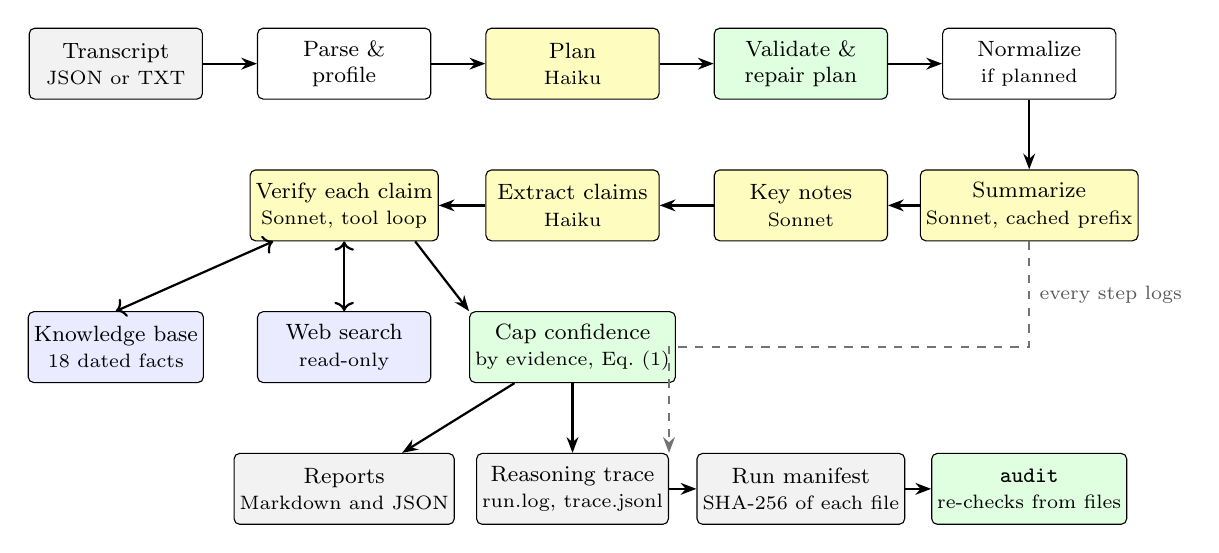
\begin{tikzpicture}[x=1cm,y=1cm,
  box/.style={draw, rounded corners=2pt, align=center, font=\footnotesize, minimum height=9mm, minimum width=22mm, inner sep=2pt, fill=#1},
  box/.default=white,
  arr/.style={-{Stealth[length=2mm]}, thick},
  lbl/.style={font=\scriptsize, text=black!65}]
% row 1: left to right
\node[box=gray!10] (in)   at (0,0)    {Transcript\\\scriptsize JSON or TXT};
\node[box]         (parse) at (2.9,0) {Parse \&\\profile};
\node[box=yellow!25] (plan) at (5.8,0) {Plan\\\scriptsize Haiku};
\node[box=green!12] (val) at (8.7,0)  {Validate \&\\repair plan};
\node[box]         (norm) at (11.6,0) {Normalize\\\scriptsize if planned};
\draw[arr] (in) -- (parse); \draw[arr] (parse) -- (plan); \draw[arr] (plan) -- (val); \draw[arr] (val) -- (norm);
% row 2: right to left
\node[box=yellow!25] (sum)    at (11.6,-1.8) {Summarize\\\scriptsize Sonnet, cached prefix};
\node[box=yellow!25] (notes)  at (8.7,-1.8)  {Key notes\\\scriptsize Sonnet};
\node[box=yellow!25] (claims) at (5.8,-1.8)  {Extract claims\\\scriptsize Haiku};
\node[box=yellow!25] (ver)    at (2.9,-1.8)  {Verify each claim\\\scriptsize Sonnet, tool loop};
\draw[arr] (norm) -- (sum); \draw[arr] (sum) -- (notes); \draw[arr] (notes) -- (claims); \draw[arr] (claims) -- (ver);
% row 3: the verifier's tools and the cap
\node[box=blue!8]  (kb)  at (0,-3.6)   {Knowledge base\\\scriptsize 18 dated facts};
\node[box=blue!8]  (web) at (2.9,-3.6) {Web search\\\scriptsize read-only};
\node[box=green!12] (cap) at (5.8,-3.6) {Cap confidence\\\scriptsize by evidence, Eq.~(1)};
\draw[arr, <->] (ver.south west) ++(0.3,0) -- (kb.north);
\draw[arr, <->] (ver) -- (web);
\draw[arr] (ver.south east) ++(-0.3,0) -- (cap.north west);
% row 4: what a run leaves behind
\node[box=gray!10]  (rep)   at (2.9,-5.4)  {Reports\\\scriptsize Markdown and JSON};
\node[box=gray!10]  (trace) at (5.8,-5.4)  {Reasoning trace\\\scriptsize run.log, trace.jsonl};
\node[box=gray!10]  (man)   at (8.7,-5.4)  {Run manifest\\\scriptsize SHA-256 of each file};
\node[box=green!12] (audit) at (11.6,-5.4) {\texttt{audit}\\\scriptsize re-checks from files};
\draw[arr] (cap) -- (rep);
\draw[arr] (cap) -- (trace);
\draw[arr] (trace) -- (man); \draw[arr] (man) -- (audit);
\draw[arr, dashed, black!55] (sum.south) |- node[lbl, pos=0.25, right]{every step logs} (9.9,-3.6) -| (trace.north east);
\end{tikzpicture}
\caption{One run of the agent. Yellow steps call a model; green boxes are deterministic code that constrains them. The plan decides which steps run (normalization was skipped for the three clean JSON transcripts in the committed Claude run), the summary strategy, the claim budget and the fact-checker's tool budget.}\label{fig:pipeline}
\end{figure}

\subsection{Planning with a validator}\label{sec:plan}
The planner (Claude Haiku~5.5) reads a profile of the transcript (length, speakers, filler and repetition counts, capitalized terms, years and prediction cues) and chooses which of five steps to run, single-pass or map-reduce summarization, a claim budget (3--8), which tools the fact-checker may use, and a budget of 2--6 tool calls per claim. Four of the five steps are required deliverables, so in practice the plan's freedom is whether to normalize the transcript and how large the claim and tool budgets are. A deterministic validator repairs missing or misordered required steps, and a fallback plan exists if planning fails outright; unit tests exercise both, and every plan in the committed Claude run was valid as written. In the committed Claude run the planner skipped transcript normalization for the three clean JSON transcripts and kept it for the one text transcript full of fillers and stutters.

\subsection{Structured outputs and failure isolation}
Every model output is validated against a schema and against business rules (for example, summary length and exactly five takeaways). On failure the specific problems are fed back to the model, for up to three attempts. The first attempt that passes every check is accepted. If none passes but at least one parsed and fit the schema, the last such output is kept with a warning, so the business rules are best-effort rather than guaranteed. Only when no attempt parsed does the step fail, and then it is isolated: steps that depend on it are skipped, independent steps still run, and the report is written with warnings. The plan and the verdicts are the two places with deterministic fallbacks: a fallback plan, and \U{} for a person to review.

\subsection{Evidence-capped verification}\label{sec:verify}
Claim verification follows the reason-act pattern of tool-using agents~\citep{yao2023react}, in the spirit of evidence-based fact verification~\citep{thorne2018fever}. The verifier is instructed to query a local knowledge base of 18 dated facts first and web search when the evidence is thin or time-sensitive; these two read-only tools are the only ones it can call. Search is a fixed mock index in every run reported here, and it is also the chart's default (\gh{73}). The verifier asks for the evidence identifiers each verdict relies on and rejects an uncited verdict up to twice; after that the verdict is kept and capped as model knowledge. The confidence the model proposes is then capped in code:
\begin{equation}
c = \min\bigl(\hat c,\ \kappa(v, S)\bigr),\qquad
\kappa(v,S)=\begin{cases}
0.50 & v=\U{},\\
0.60 & S=\varnothing\ \text{(model knowledge only)},\\
0.90 & |S|=1,\\
0.95 & |S|\ge 2\ \text{(both source types cited)},
\end{cases}
\end{equation}
where $\hat c$ is the model's confidence, $v$ the verdict and $S$ the set of source types cited. Two source types cited is not two independent sources: the knowledge base and the mock index were written by the same author from the same facts, and in the live run the 0.95 tier never bound. When the loop ends without a valid verdict, the claim gets \U{} at 0.20 for a person to review. A claim the extractor typed as a prediction is \U{} while its deadline is ahead, enforced after the model's verdict. That rule exists because the first real bug was its absence: an unexpired prediction marked \Ou{} instead of \U{} (\gh{13}). Its deadline test still has a gap: it treats any past year in the claim as the deadline, so a prediction that mentions a past baseline year (``by 2030, double its 2020 level'') escapes the rule (\gh{71}).

\subsection{Reasoning trace, caching and audit}
Every plan, tool call with its stated purpose, observation, self-correction and verdict is written twice: as a readable log and as structured JSON lines carrying the run, episode, step and OpenTelemetry trace and span identifiers. The run manifest records the code commit, prompt version, settings, per-step timings, token usage, and SHA-256 hashes of every input, report and the structured trace. A separate \code{audit} command re-checks a finished run from those files alone: hashes, the plan, summary length, every quote re-matched to its line ($\ge$0.90), every claim grounded in its transcript line, and every confidence within its evidence cap. The committed Claude run passes all 36 of its audit checks. These are checks of integrity and consistency, not of correctness: that run still contains the \gh{13} error, the manifest is unsigned, and it was produced by v0.1.0 code at a commit renamed by a later history rewrite (the mapping is committed). For cost, the transcript is a cacheable prefix that later steps read back at 5\% of the input price; in the committed run the cache was already warm, so its measured costs are warm-cache figures.

\section{Evaluation}\label{sec:eval}

\subsection{Datasets, metrics and gates}
The fact-check dataset has 25 labeled claims tagged by case type (verified fact, stale fact, contradicted, future deadline, passed deadline, no deadline, anecdote, ambiguous, and three regression cases for \gh{13}). We report verdict accuracy, macro-F1, citation validity (the share of \V{} and \Ou{} verdicts that cite at least one item a tool returned; identifiers that were not retrieved are stripped before scoring), the Brier score~\citep{brier1950} and expected calibration error (ECE)~\citep{guo2017calibration}. Per-episode expectations cover summary length and coverage of required themes, the shape of the notes, quote fidelity, claim recall and claim-verdict accuracy. A rubric judge (Claude Sonnet~5.5, following the LLM-as-a-judge approach~\citep{zheng2023judging}) grades each summary for faithfulness (weight 0.5), coverage (0.3) and concision (0.2), and lists statements the transcript does not support; each such statement costs 0.15, loosely inspired by atomic factual-precision scoring~\citep{min2023factscore}. Theme coverage is a case-insensitive keyword match, and claim precision is not measured.

Two suites use these. The \emph{offline} suite runs on every pull request with a deterministic provider, so it cannot see prompts. Eight of its 19 gates run the labeled claims through heuristics; the other eleven re-score committed runs, so they guard the scorers and the committed artifacts, not the agent's code. Its thresholds are a ratchet set at the values achieved, the caps of Eq.~(1) never bind on the heuristic's output, and the heuristic returns \U{} for pending predictions before the \gh{13} rule runs; unit tests, not this suite, cover those rules. The \emph{live} suite runs Claude on the labeled claims and on fresh runs of every bundled transcript; it is scheduled nightly and can be dispatched by hand. One live run exists, on main. Because the nightly run is not a required check, a prompt regression is found after merge, not before. A live run fails if it misses a threshold or drops more than 0.05 below its baseline.

\subsection{Results}
Table~\ref{tab:factcheck} compares the two providers on the labeled claims. The live run met all 14 of its thresholds and the offline suite all 19 of its own. Brier and ECE are computed over the verdicts that are not \U{}: 17 in the live run, 15 offline, so the two columns cover different subsets. None of the 17 live verdicts was wrong, so these scores measure how far confidence sits below 1.0, not whether it separates right answers from wrong ones; with no errors they cannot show calibration. ECE (five bins) is 0.162 with the capped confidences and 0.154 with the model's own: the caps bound only 3 of the 17 asserted verdicts (Figure~\ref{fig:caps}). The under-confidence is the model's, not the caps'.

\begin{table}[t]
\centering\small
\caption{Fact-check results on the 25 labeled claims. The offline provider is deterministic heuristics used to gate code changes; the live run used Claude Sonnet~5.5 and Haiku~5.5.}\label{tab:factcheck}
\begin{tabular}{@{}lcc@{}}
\toprule
Metric & Offline (every PR) & Live (Claude) \\
\midrule
Verdict accuracy & 0.96 & 1.00 \\
Macro-F1 & 0.916 & 1.00 \\
Citation validity & 1.00 & 1.00 \\
Brier score $\downarrow$ & 0.027 & 0.033 \\
ECE & 0.151 & 0.162 \\
Tool calls per claim & 1.08 & 1.88 \\
Thresholds met & 19/19 & 14/14 \\
\bottomrule
\end{tabular}
\end{table}

\begin{figure}[t]
\centering
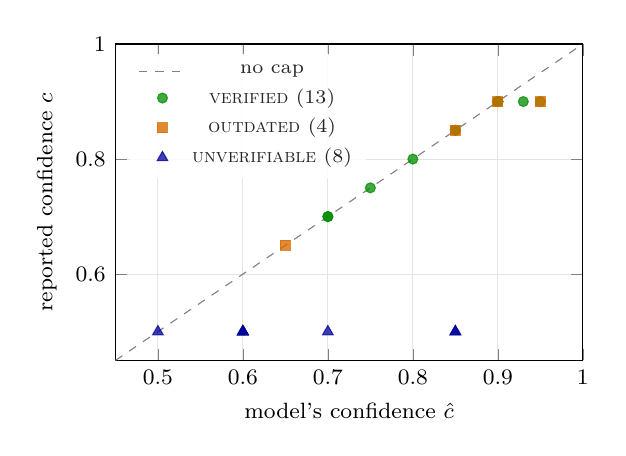
\begin{tikzpicture}
\begin{axis}[width=0.62\linewidth, height=5.6cm, xmin=0.45, xmax=1.0, ymin=0.45, ymax=1.0,
  xlabel={model's confidence $\hat c$}, ylabel={reported confidence $c$}, font=\footnotesize,
  legend style={at={(0.03,0.97)}, anchor=north west, font=\scriptsize, draw=none, fill=white, fill opacity=0.85},
  grid=major, grid style={gray!20}]
\addplot[gray, dashed, domain=0.45:1.0] {x}; \addlegendentry{no cap}
\addplot[only marks, mark=*, mark size=1.8pt, color=green!55!black, opacity=0.75] coordinates {
  (0.95,0.90) (0.90,0.90) (0.93,0.90) (0.90,0.90) (0.85,0.85) (0.70,0.70) (0.85,0.85) (0.90,0.90)
  (0.80,0.80) (0.70,0.70) (0.75,0.75) (0.90,0.90) (0.90,0.90)};
\addlegendentry{\V{} (13)}
\addplot[only marks, mark=square*, mark size=1.8pt, color=orange!85!black, opacity=0.8] coordinates {
  (0.90,0.90) (0.95,0.90) (0.65,0.65) (0.85,0.85)};
\addlegendentry{\Ou{} (4)}
\addplot[only marks, mark=triangle*, mark size=2.2pt, color=blue!60!black, opacity=0.75] coordinates {
  (0.60,0.50) (0.60,0.50) (0.60,0.50) (0.50,0.50) (0.60,0.50) (0.85,0.50) (0.85,0.50) (0.70,0.50)};
\addlegendentry{\U{} (8)}
\end{axis}
\end{tikzpicture}
\caption{What the evidence caps of Eq.~(1) did in the live run: each of the 25 labeled claims, by the confidence the model proposed and the confidence reported. Points on the diagonal were not capped. The caps bound 3 of the 17 asserted verdicts (\V{} or \Ou{}, all correct) and 7 of the 8 \U{} verdicts, which are capped at 0.50 by definition. Points overlap where values coincide.}\label{fig:caps}
\end{figure}

Table~\ref{tab:episodes} shows the live run's fresh episodes. Every summary was in range and covered its required themes, every quote matched its line, and every expected claim was found and judged correctly. Three of four summaries scored 0.95 with the judge. The fourth, ep004, scored 0.475 because the judge listed two statements as unsupported; we return to it in \S\ref{sec:judge}. Note the source lengths: three of the four summaries are longer than the transcripts they summarize, because the brief asks for 200--300 words and the bundled transcripts run 122--325.

\begin{table}[t]
\centering\small
\caption{Live run, fresh episodes. Judge sub-scores are faithfulness (F), coverage (C) and concision (K) on a 1--5 scale.}\label{tab:episodes}
\setlength{\tabcolsep}{4.5pt}
\begin{tabular}{@{}lcccccccl@{}}
\toprule
Episode & Source & Summary & Coverage & Quotes & Claims & Verdicts & Judge \\
 & words & words & & matched & found & right & \\
\midrule
ep001 & 325 & 269 & 1.00 & 5/5 & 2/2 & 2/2 & 0.95 (F5 C5 K4) \\
ep002 & 233 & 282 & 1.00 & 5/5 & 3/3 & 3/3 & 0.95 (F5 C5 K4) \\
ep003 & 192 & 270 & 1.00 & 5/5 & 2/2 & 2/2 & 0.95 (F5 C5 K4) \\
ep004 & 122 & 219 & 1.00 & 4/4 & 5/5 & 5/5 & 0.475 (F4 C5 K3), 2 flagged \\
\bottomrule
\end{tabular}
\end{table}

\paragraph{What these numbers can and cannot show.} They are regression gates for this system, not estimates of how it would do on a client's episodes, and the reasons are specific. The knowledge base and the mock index were written for exactly these claims: each of the 13 verified-fact claims has its own knowledge-base entry, and the prompt calls the knowledge base trusted. A regex baseline scores 0.96 on the same 25 claims, partly because its contradiction cues echo the knowledge base's wording. Five of the 25 claims are decided by code once the claim is typed as a prediction, so the model decided 20, and got 20 right: a 95\% confidence interval of [0.83, 1.00] (Clopper--Pearson). There is one live run, of a model that takes no temperature setting, so run-to-run variation is unmeasured. And the transcripts are 122--325 words long. Held-out claims labeled by someone else, checked against an untailored knowledge base or real search, with three or more runs, are the next step (\S\ref{sec:limits}).

\subsection{Evaluating the evaluator}\label{sec:judge}
The judge's first flagged statement in ep004 was ``Chris Bell is the host and Nina Alvarez is the guest (roles not stated in the transcript).'' The roles are stated in the transcript's header, and every agent step sees them on each line (\code{[00:02:14] Chris Bell (host): \ldots}). The judge, however, rendered its own copy of the transcript with speaker names only. The agent was right and the judge was wrong: the judge had been given less information than the system it graded. The fix gives the judge the same rendering the agent sees, with a regression test that the judge's prompt carries the roles (\gh{51}, root cause addressed in pull request \#62). The second flag, that the summary ``editorializes'', is plausibly right: the summary is 219 words for a 122-word transcript, and the 200-word floor pushes the model to pad; the committed run's ep004 summary ends with a line telling listeners they will find ``a brief, accessible overview here''. An adaptive length mode exists for very short episodes but is off by default. The judge is also Sonnet grading Sonnet, and LLM evaluators are known to favor their own generations~\citep{panickssery2024}; the judge's version is not yet recorded in the evaluation output.

The lesson generalizes. An LLM judge is code with inputs, and when it disagrees with the system under test, either side may be wrong, here one flag each way. Gates measure the failures one anticipated; an open-ended judge surfaces new ones, including its own.

\subsection{Cost}
The deployment model estimates about \$0.17 for an hour-long episode with ten claims at list prices (Sonnet~5.5 at \$2 and \$10 per million input and output tokens; Haiku~5.5 at \$0.10 and \$0.50; cache reads at 5\% of input). Measured on the committed Claude run, from per-call token counts in its trace at the same prices, the four sample episodes cost \$0.100, \$0.051, \$0.054 and \$0.068 (Figure~\ref{fig:cost}).\footnote{Cache writes are counted as input at the base price; the 25\% write surcharge is not, and this warm-cache run wrote none. A cold run adds roughly \$0.002--\$0.003 per sample episode.} Verification accounted for 75\% of the spend, summary and notes for 24\%, and planning and claim extraction for under 1\% each. The same pricing now runs inside the agent, per call (\S\ref{sec:drill}). Verification is therefore the first cost lever. Running the claim loop on Haiku and escalating to Sonnet only for \Ou{} or low-confidence verdicts would bring the modeled episode to about \$0.09, assuming 30\% of verdicts escalate and Haiku verdicts are as accurate, which is untested; and that rule never re-checks a confident wrong \V{}, the costliest error. At 500 episodes a month, model spend is under \$100; we have not measured infrastructure cost, but a managed cluster alone likely exceeds that.

\begin{figure}[t]
\centering
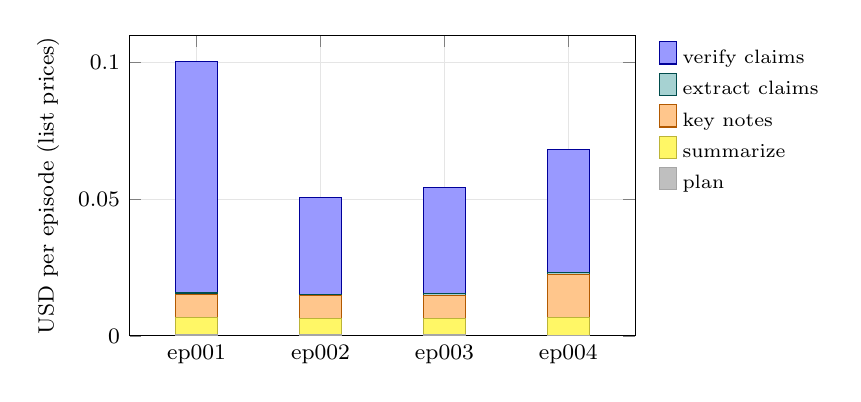
\begin{tikzpicture}
\begin{axis}[ybar stacked, bar width=15pt, width=0.66\linewidth, height=5.4cm, ymin=0, ymax=0.11,
  ylabel={USD per episode (list prices)}, symbolic x coords={ep001,ep002,ep003,ep004}, xtick=data,
  font=\footnotesize, yticklabel style={/pgf/number format/fixed, /pgf/number format/precision=2},
  legend style={at={(1.03,1)}, anchor=north west, font=\scriptsize, draw=none}, legend cell align=left, reverse legend,
  grid=major, grid style={gray!20}, enlarge x limits=0.18]
\addplot[fill=gray!50, draw=gray!70] coordinates {(ep001,0.0004) (ep002,0.0004) (ep003,0.0004) (ep004,0.0003)};
\addlegendentry{plan}
\addplot[fill=yellow!60, draw=yellow!70!black] coordinates {(ep001,0.0064) (ep002,0.0059) (ep003,0.0061) (ep004,0.0063)};
\addlegendentry{summarize}
\addplot[fill=orange!45, draw=orange!70!black] coordinates {(ep001,0.0082) (ep002,0.0086) (ep003,0.0084) (ep004,0.0159)};
\addlegendentry{key notes}
\addplot[fill=teal!35, draw=teal!60!black] coordinates {(ep001,0.0007) (ep002,0.0003) (ep003,0.0005) (ep004,0.0007)};
\addlegendentry{extract claims}
\addplot[fill=blue!40, draw=blue!60!black] coordinates {(ep001,0.0848) (ep002,0.0355) (ep003,0.0389) (ep004,0.0451)};
\addlegendentry{verify claims}
\end{axis}
\end{tikzpicture}
\caption{Measured cost of the committed Claude run by step, priced per call from its trace (Sonnet~5.5 \$2/\$10 and Haiku~5.5 \$0.10/\$0.50 per million input/output tokens, cache reads at 5\%). Verification is 75\% of the total of \$0.274.}\label{fig:cost}
\end{figure}

\section{Engineering for operation}\label{sec:ops}

\subsection{Process and gates}
Version 0.1.0 was fourteen commits pushed directly to the main branch, with a CI workflow that nothing was required to pass. Since then every change has reached main through a pull request, with one exception: a commit recording the mapping of old to new commit identifiers after the history was rewritten on 2026-10-14 to correct authorship (proofs captured before the rewrite cite the old identifiers). Repository rulesets enforce squash-only merges, seven required checks (the PR Gate, secret scanning, workflow linting, Trivy, CodeQL for Python and for workflows, and dependency review) and no new high-severity CodeQL alert. The PR Gate covers linting, types, the unit tests with an 83\% coverage floor (85\% today), configuration drift, the offline evaluation suite, the Docker image run end to end, the Helm chart for every environment, and the observability stack end to end. Three further checks are advisory, not required: Argo~CD installing dev on a throwaway kind cluster, ClusterFuzzLite~\citep{clusterfuzzlite} fuzzing of the transcript parsers, and the nightly live evaluation.

Table~\ref{tab:defects} lists the defects found after v0.1.0 and what found them. Most would not surface in a demonstration: \gh{13} did appear on a bundled transcript, but only for someone reading the verdicts closely, and \gh{64} needed the documented quickstart with a real key.

\begin{table}[t]
\centering\small
\caption{Defects found after v0.1.0, what found them, and the fix. Numbers are issues and pull requests in the repository.}\label{tab:defects}
\begin{tabularx}{\linewidth}{@{}>{\raggedright\arraybackslash}p{0.34\linewidth}>{\raggedright\arraybackslash}p{0.24\linewidth}X@{}}
\toprule
Defect & Found by & Fix \\
\midrule
Unexpired prediction marked \Ou{} & reviewing the committed Claude run & \U{} enforced in code after the verdict, plus an eval case (\gh{13}) \\
Transcript-supplied episode ids could write outside the output folder & security review for the Best Practices criteria & ids reduced to a safe alphabet, with a regression test (\gh{24}) \\
Argo~CD project blocked the namespace the deployment creates & Argo~CD on a throwaway kind cluster in CI & namespace allowed in the project (pull request \#36) \\
Header regex backtracked quadratically on crafted input & CodeQL, a required check, once transcripts became API input & value must start with a non-space (\code{py/polynomial-redos}) \\
Malformed JSON transcript $\to$ HTTP 500 & fuzzing, within seconds & typed errors, HTTP 422 (\gh{49}) \\
Judge saw names without roles & following up a judge flag & judge gets the agent's rendering (\gh{51}, \#62) \\
Prod network policy blocked telemetry & fact-checking this paper & egress to the Collector's port (\gh{61}, \#63) \\
Docker quickstart failed with an API key & fact-checking this paper & example env no longer overrides the cache path (\gh{64}, \#65) \\
Prediction mentioning a past year escapes the deadline rule & red-teaming this paper & open (\gh{71}) \\
Quotes kept in the model's wording, not the transcript's & red-teaming this paper & open (\gh{72}) \\
Production inherits mock web search & red-teaming this paper & open (\gh{73}) \\
API and worker keep no audit trail & red-teaming this paper & open (\gh{74}) \\
Two alert rules had no unit test, though documented as tested & red-teaming this paper & promtool tests for all seven rules (\#75) \\
\bottomrule
\end{tabularx}
\end{table}

\subsection{Supply chain: build once, promote by digest}
Each code merge builds one multi-architecture image (amd64 and arm64) with a software bill of materials and SLSA build provenance~\citep{slsa}; the provenance is a GitHub attestation signed through Sigstore~\citep{newman2022sigstore}, while the SBOM is attached unsigned, so the build meets SLSA Build Level~2. Nothing is rebuilt for production: a release re-tags the digest that main built, and promotion is a small pull request that changes the tag and digest. Two qualifications matter. The PR Gate tests a separate amd64 build of the same commit, not the published multi-arch digest, and arm64 is not tested in CI; and the release workflow checks that the digest exists, not that dev ran it. At the v0.2.0 release, development and production were pinned to the same digest (\code{sha256:67a18fc8\ldots}); no cluster ran either at the time. Anyone can verify the provenance without a registry login using \code{gh attestation verify}, or against the Sigstore bundle attached to the release (a fully offline verification has not been demonstrated). This maps directly to practices PS.2 and PS.3 of NIST's Secure Software Development Framework~\citep{nist2022ssdf}. The OpenSSF Scorecard~\citep{scorecard} is 7.7, and the Best Practices badge~\citep{bestpractices} is at the passing level with all 67 criteria met or not applicable.

\subsection{GitOps delivery}
The Helm chart deploys an API with a horizontal autoscaler and disruption budget, queue workers scaled by KEDA on queue depth, an ExternalSecret for API keys, a NetworkPolicy, and a service account ready for IAM roles for service accounts. An Argo~CD~\citep{argocd} ApplicationSet renders it per environment: development syncs automatically from main, and production waits for a person to press Sync. The two environments are namespaces in one cluster, and both render the chart from main; only the image is pinned per environment, so a production Sync applies the current chart with production's image. Figure~\ref{fig:delivery} shows the path from a pull request to a running pod.

\begin{figure}[t]
\centering
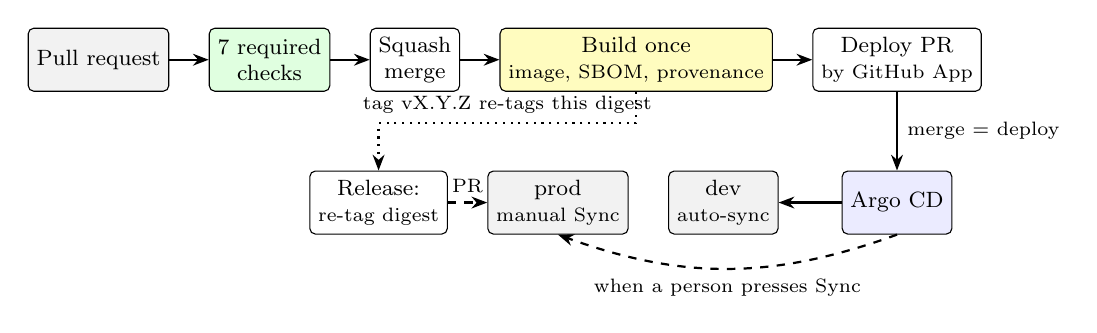
\begin{tikzpicture}[
  box/.style={draw, rounded corners=2pt, align=center, font=\footnotesize, minimum height=8mm, inner sep=3pt, fill=#1},
  box/.default=white,
  arr/.style={-{Stealth[length=2mm]}, thick}]
\node[box=gray!10] (pr) {Pull request};
\node[box=green!12, right=5mm of pr] (gate) {7 required\\checks};
\node[box, right=5mm of gate] (merge) {Squash\\merge};
\node[box=yellow!25, right=5mm of merge] (pub) {Build once\\\scriptsize image, SBOM, provenance};
\node[box, right=5mm of pub] (dpr) {Deploy PR\\\scriptsize by GitHub App};
\draw[arr] (pr) -- (gate); \draw[arr] (gate) -- (merge); \draw[arr] (merge) -- (pub); \draw[arr] (pub) -- (dpr);
\node[box=blue!8, below=10mm of dpr] (argo) {Argo CD};
\node[box=gray!10, left=8mm of argo] (dev) {dev\\\scriptsize auto-sync};
\node[box=gray!10, left=5mm of dev] (prod) {prod\\\scriptsize manual Sync};
\node[box, left=5mm of prod] (rel) {Release:\\\scriptsize re-tag digest};
\draw[arr] (dpr) -- node[right, font=\scriptsize]{merge = deploy} (argo);
\draw[arr] (argo) -- (dev);
\draw[arr, dashed] (rel) -- node[above, font=\scriptsize]{PR} (prod);
\draw[arr, dotted] (pub.south) -- ++(0,-4mm) -| node[pos=0.25, above, font=\scriptsize]{tag vX.Y.Z re-tags this digest} (rel.north);
\draw[arr, dashed] (argo.south) to[bend left=20] node[below, font=\scriptsize]{when a person presses Sync} (prod.south);
\end{tikzpicture}
\caption{Delivery. One image is built per merge and promoted by digest; a release re-tags it. Deploy pull requests pass the same seven checks and are opened by a GitHub App, because pull requests opened with a workflow's own token do not trigger checks. Both environments render the chart from main, in one cluster.}\label{fig:delivery}
\end{figure}

A standing lab cluster (kind on a Mac mini, reached over Tailscale with its own kubeconfig) makes this measurable. For one deploy pull request (\#55), the merge landed at 12:46:35Z, Argo~CD started an automated sync at 12:47:18Z, 43\,s later, and by 12:47:48Z the service's health endpoint reported the new commit. The lab polls Git every 30\,s (Argo~CD's default is 180\,s), which bounds that figure. No one ran \code{kubectl}. An advisory CI check installs the same Argo~CD configuration on a throwaway kind cluster for every deployment change. Measuring a sync needs care: a watcher has to wait for a ready pod and a Synced, Healthy application before it watches for the image to change, or it reports a sync that has not happened.

\subsection{Observability}
With telemetry on, every run is one OpenTelemetry trace (production samples a quarter of traces): a root \code{run} span, an \code{invoke\_agent} span per episode, a span per plan step, a \code{verify\_claim} span per claim, and \code{chat} and \code{execute\_tool} spans for model and tool calls. Names and \code{gen\_ai.*} attributes follow the GenAI semantic conventions~\citep{otelgenai}, so backends understand them without custom parsing. By default spans carry identifiers, counts, model names, token usage, durations and verdicts, and no transcript, claim, prompt or completion text; content capture is an explicit opt-in for local debugging. Seven alert rules each have \code{promtool} unit tests, including cases where they must stay quiet; until the fact-check of this paper, two of them had only a syntax check.

The agent exports once, over OTLP, to an OpenTelemetry Collector whose traces pipeline has two exporters: Jaeger, which answers where the time went, and MLflow~\citep{mlflowotel}, which reads the GenAI attributes and presents each run as an agent trace with typed spans (\code{invoke\_agent} becomes AGENT, \code{chat} becomes CHAT\_MODEL, \code{execute\_tool} becomes TOOL) and token totals (Figure~\ref{fig:mlflow}). The second backend required no agent code. The edges took the work: MLflow needs a SQL store to ingest OTLP, it rejects unrecognized Host headers to defend against DNS rebinding, and macOS reserves its default port. The integration was prompted by a community talk on agents in production~\citep{fluckiger2026}. The lab cluster now runs the same pipelines in Kubernetes, deployed by Argo~CD: Jaeger, Prometheus and Alertmanager, and a private MLflow from its official chart with a Postgres store and basic authentication, where the Collector writes as its own user with edit rights on one experiment and nothing else.

\begin{figure}[t]
\centering
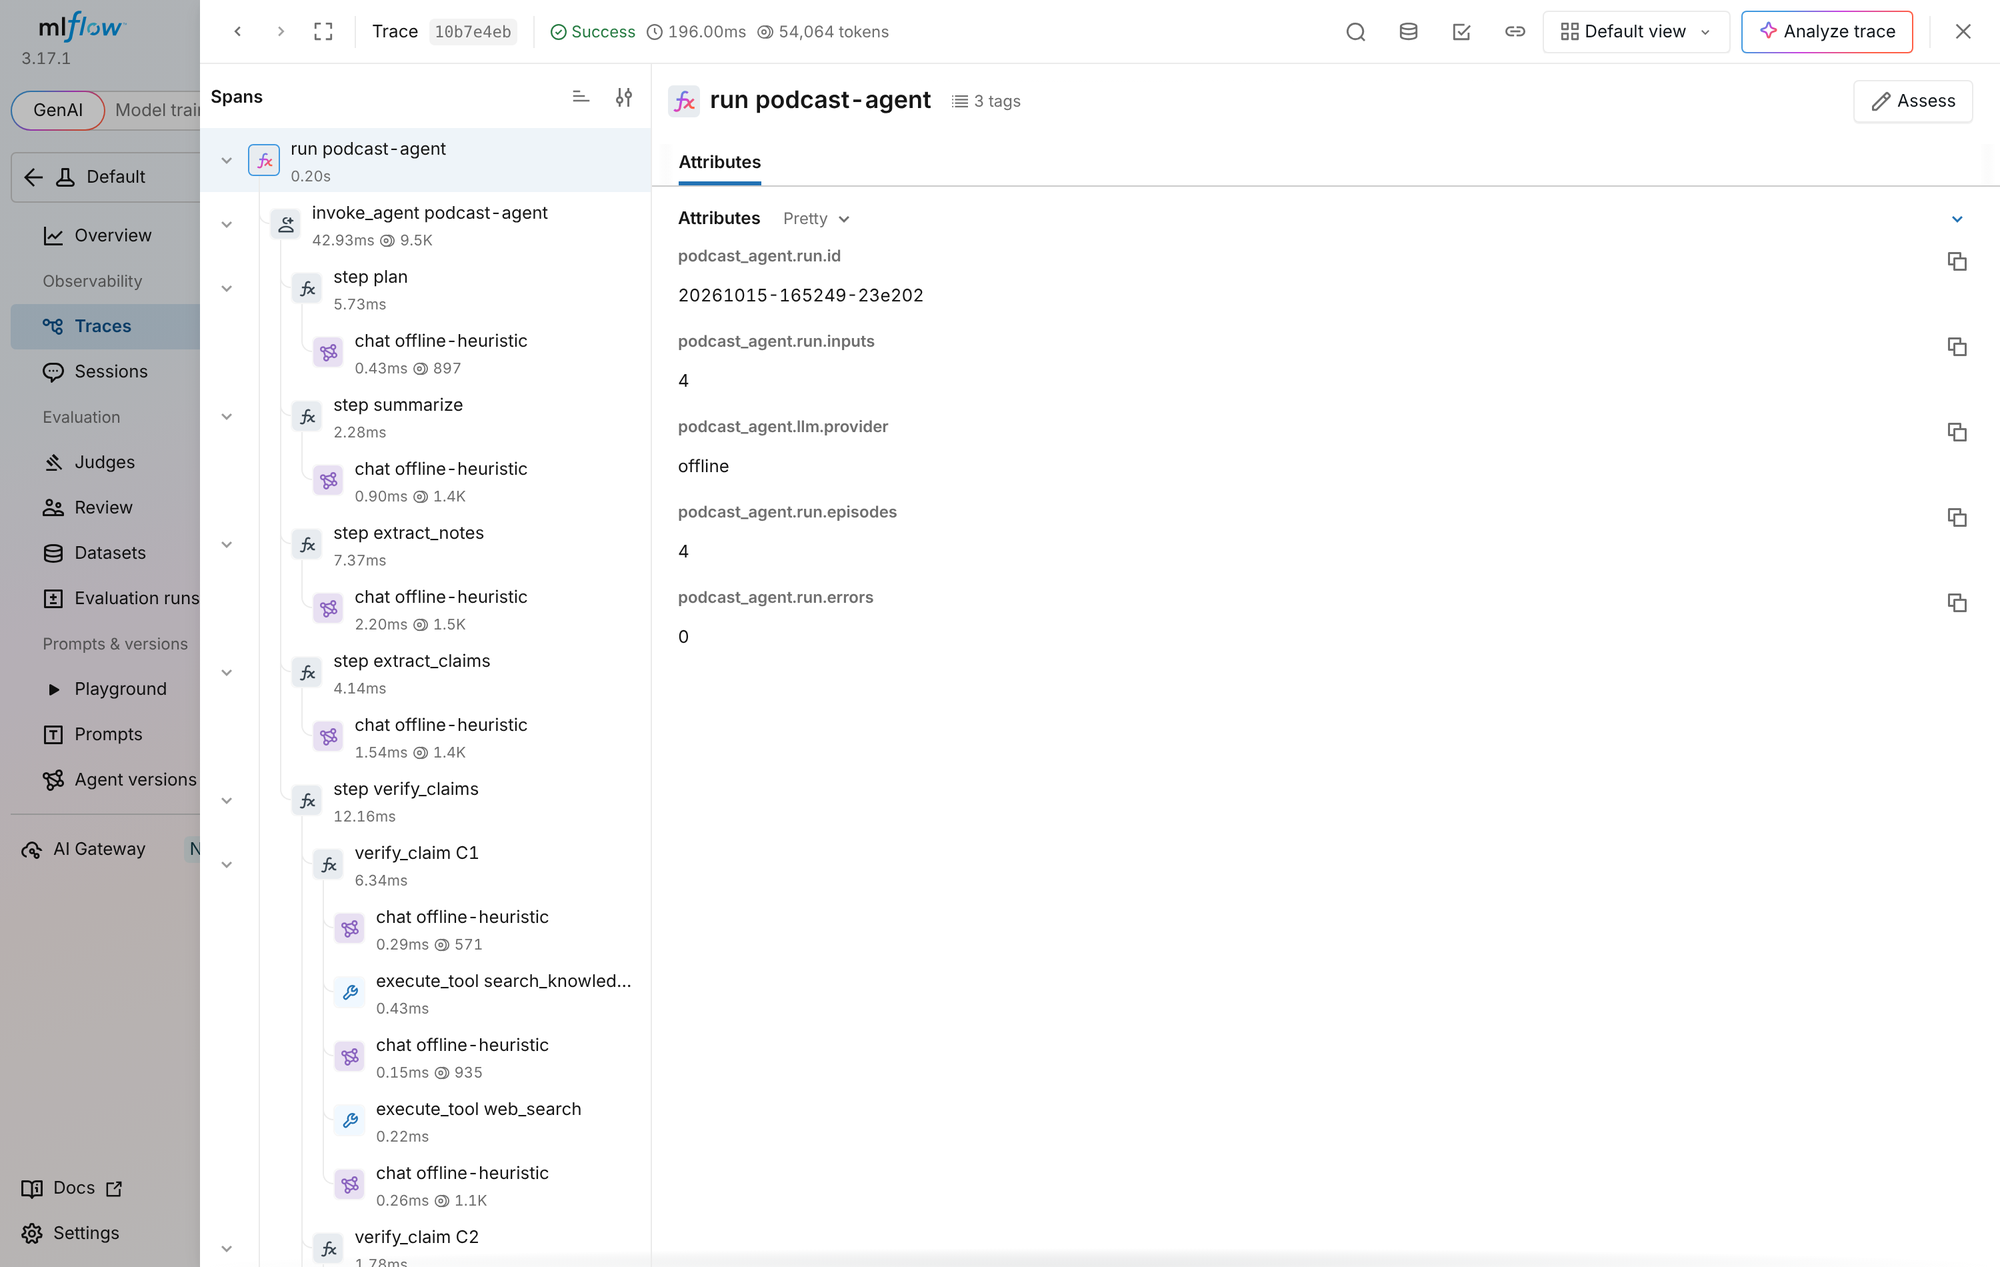
\includegraphics[width=0.86\linewidth]{figures/mlflow-trace.png}
\caption{One trace in MLflow, for an offline run of all four episodes: 196\,ms and 54{,}064 tokens (offline token counts are estimates). The span tree runs from \code{run podcast-agent} through \code{invoke\_agent}, each step and \code{verify\_claim}, to \code{chat} and \code{execute\_tool}. The 128-span count that both backends held was checked on a run of identical inputs.}\label{fig:mlflow}
\end{figure}

Each exporter has its own queue and retries, so one backend's failure should not hold up the other. CI checks this on every pull request: it stops MLflow, runs an episode, confirms that Jaeger received the whole trace, restarts MLflow, and confirms that the Collector's retry delivered every queued span. On a full run both backends held 128 of 128 spans; in the outage test, one 37-span episode during a short outage, the queued spans arrived after the restart. That is the case CI shows, not a general guarantee: the queues live in memory, so a Collector restart loses both copies; retries give up after five minutes; and the two exporters share the pipeline's memory limiter, so a long MLflow backlog could eventually refuse data meant for Jaeger too.

\subsection{Security for regulated deployments}
The software is open source, not a service; it holds no FedRAMP authorization and runs inside a deploying organization's authorization boundary. The repository's security policy maps 14 practices of NIST SSDF~1.1~\citep{nist2022ssdf} to evidence in the repository and gives configuration for that boundary: model traffic that stays in AWS under the customer's IAM (Bedrock) or on a self-hosted model; verification with a local model and the local knowledge base only; telemetry that stays inside the boundary with content capture off; deployment by digest; and an audit trail per run. Several of these are configuration and advice rather than enforcement, and the gaps should be stated as plainly. Provenance is verified by hand, not by an admission controller. The in-boundary model paths are the least tested: Bedrock only with mocks, the OpenAI-compatible provider not at all. The audit trail exists only for CLI runs (\gh{74}), and the chart's default search is the mock index (\gh{73}). Prompt injection~\citep{greshake2023,owasp2025llm} is mitigated only by structure: the verifier can call just two read-only tools and every output is schema-checked, but the prompts carry no injection guard, network egress allows HTTPS to any host, and none of the evaluation cases is adversarial. A malicious transcript or page could sway a verdict, the summary or the notes, which a person reviews, and with real search enabled the model-written query is a channel to a third party. The policy also states what is absent: no authentication or rate limits on the HTTP API itself (it belongs behind the customer's gateway), and a base image that is not FIPS-validated.

\section{Cost control, detected before the customer}\label{sec:drill}
DRILLSECTION

\section{Self-audit: fact-checking the write-up}\label{sec:selfaudit}

We checked this paper against the repository twice. The first pass compared each statement in an earlier draft with the code, the captured proofs and the repository history, and corrected a dozen overstatements: describing a low Brier score as ``calibrated''; calling the judge advisory when two live gates depend on it; claiming that the offline suite catches prompt regressions, which it cannot, since the offline provider ignores prompts; quoting a modeled cost as a measured one; ``five steps'' where the planner had chosen four; and a release-time digest described as current. It also found two real defects. The production values enabled telemetry to the Collector on port 4318 while the chart's NetworkPolicy allowed egress only on ports 53 and 443, so production would have silently dropped its traces and metrics (\gh{61}). And the documented Docker quickstart failed at the first model call when given an API key, because the example environment file overrode the image's cache directory with one the container user cannot create (\gh{64}); offline runs never build the cache, which is why CI missed it.

The second pass was adversarial: a separate model instance, working read-only and instructed to find every statement the repository does not support and every objection a skeptical reviewer would raise, recomputed the numbers it could (costs, Brier, ECE, judge scores, gate counts, span counts) and checked 219 statements. It confirmed the measured numbers and found 83 problems. Most were overstatements now corrected in the text above, including our own claim to have ``checked every number''. Four were production-path gaps now filed as issues (\gh{71}--\gh{74}), and one was a documentation claim that was simply false (two alert rules called unit-tested had no test, fixed in \#75). Its largest objection, that the evaluation is effectively an answer key, is now stated in \S\ref{sec:eval}. The narrative is itself an artifact, and it is worth testing like one, more than once.

\section{Lessons}\label{sec:lessons}
\begin{enumerate}[leftmargin=*]
  \item \textbf{Build to the specification first, then make it operable.} A working demonstration answers whether it can be done; a customer needs to run it, trust it and change it safely.
  \item \textbf{Let the model plan, but never let the run depend on it.} The model decides; code validates, repairs, retries and isolates.
  \item \textbf{Bound confidence by evidence, and check whether the bound binds.} Caps tied to the evidence gathered keep a verdict honest, but in the live run they bound only 3 of 17 asserted verdicts; the rest was the model's own confidence.
  \item \textbf{Evaluate the evaluator.} A judge needs the same inputs as the system it grades, and tests of its own.
  \item \textbf{A check nobody is required to pass is not a gate.} Required checks turned claims into evidence and found bugs a demonstration would not; by this standard the Argo~CD install, fuzzing and the nightly live run are still advisory.
  \item \textbf{The thing you tested should be the thing you ship.} Build once, promote by digest, and let anyone verify the provenance. Here that holds for the image; the chart and configuration still come from main.
  \item \textbf{Measure readiness before you measure change.} Proving automation takes the same care as building it.
  \item \textbf{If the agent only speaks OTLP, a new backend is a configuration change}, and failure isolation between backends can be tested in CI.
  \item \textbf{For a regulated customer, security is evidence, not adjectives}, including a plain statement of what is missing.
  \item \textbf{Fact-check the story too, and then red-team it.} Two defects in Table~\ref{tab:defects} came from checking this write-up, and an adversarial second pass found five more problems the first had passed over.
  \item \textbf{Detect it before the customer does.} A synthetic canary that runs the most expensive kind of episode every minute turned a cost regression into a ticket naming the change, while no customer episode had yet gone over budget.
  \item \textbf{Let the measurements choose the next step.} The cost model, the evaluations and the drill's timeline, not a feature list, set the roadmap.
\end{enumerate}

\section{Limitations and future work}\label{sec:limits}
\textbf{Small, purpose-built evaluation sets.} Twenty-five labeled claims and four episodes gate regressions in this system but do not estimate accuracy in general: the knowledge base and mock index were written for these claims, the transcripts are 122--325 words, there is one live run, and no case is adversarial. A production deployment needs a client-specific labeled set, labeled by someone other than the builder and refreshed as the knowledge base changes. \textbf{Mock search}, in every run reported here and in the chart's default configuration (\gh{73}); real search adds latency, noise and new failure modes. \textbf{A single judge model}, of the same family as the system it grades; a second judge or periodic human agreement checks would bound its error. \textbf{No audit trail on the production path} (\gh{74}), and no latency figures: the committed run took 3.5 minutes for four short episodes. \textbf{One maintainer.} No change has had a second reviewer, which the OpenSSF Scorecard reports and which tooling cannot fix; the repository's age and contributor diversity are similar. \textbf{Not yet run on AWS.} The chart's AWS components (KEDA on SQS, ExternalSecrets, IAM roles for service accounts) are rendered and schema-checked on every change, and the GitOps flow runs on kind, but the AWS path has not been exercised. Provider failover through a model gateway, queue redrive and multi-region recovery are designed, not built. \textbf{The cost drill ran in a lab}, against the offline provider with list-price estimates; its timings include CI and a human merge, which is the point, but a production incident would add paging and a reviewer who is not the author.

Next steps follow the measurements: the four open issues from the second fact-check; held-out, independently labeled claims and repeated live runs; tiered verification; the drill's follow-ups, starting with a CI check that prices a configuration change before it merges; the nightly judge's scores attached to each run's trace; a model gateway with per-tenant budgets, rate limits and failover; and audio or video input through a speech-to-text step with speaker labels, ahead of a pipeline that otherwise does not change.

\section{Conclusion}
A fact-checking agent is only as useful as the trust its users can place in it, and that trust is built mostly outside the model: in validators and evidence caps, in evaluations that gate every change, in a delivery path where the tested image is the shipped image, in telemetry that keeps flowing when one backend is down, and in alerts that reach a person with the evidence before a customer notices. The most instructive findings came from treating every component as testable, including the judge, the narrative and the response to an incident.

\section*{Acknowledgments}
Thanks to the mentor whose review of v0.1.0 set the agenda for v0.2.0, and to Joseph Fluckiger, whose AIMUG talk prompted the MLflow integration. The second fact-check pass was performed by a separate instance of Claude working read-only. The agent's model calls use Anthropic's Claude Sonnet~5.5 and Haiku~5.5.

\bibliographystyle{plainnat}
\bibliography{references}

\end{document}
